\documentclass[10pt]{examdesign}
\usepackage{amsmath}
\usepackage{enumitem}
\usepackage{amsfonts}
\usepackage{pgfplots}
\usepackage{pifont}
\usepackage{graphicx}
\usepackage{fancyhdr}
\usepackage{cancel}
\usepackage{gensymb}
\usepackage[american]{circuitikz}

\SectionFont{\large\sffamily}
\Fullpages
\ContinuousNumbering
\usepackage{ulem}
\ProportionalBlanks{2}


\DefineAnswerWrapper{}{}
\NumberOfVersions{1}
%\IncludeFromFile{foobar.tex}
\examname{\Large{Universal Gravitation}}
\class {\Large Physics}

\def \namedata {Name: \hrulefill\\ 
	Date: \hrulefill \\
	Period: \hrulefill \\
	Primary Peer Reviewer: \hrulefill 
	\\
			\begin{tabular}{| p{1cm} | p{1cm} | p{1 cm} | p{1cm} |}
	\hline
		+1 & 0 & -1 & $\Sigma$ 
		\\
		\hline
		& & & \vspace{.5cm}
		\\ \hline
	
	\end{tabular}
	\\
 \vspace{-.6in}
	
}




\begin{document}




\begin{multiplechoice} [title={Multiple Choice},
	rearrange=no]

\textit{For Each question, choose the best answer.}

	Some Formulas: 
	\begin{center}
	$F_c = \frac{mv^2}{r} $	\hspace{1 in} $F_g = \frac{Gm_1m_2}{r^2}$ \hspace{1in} $G = 6.67\times 10^{-11}Nm^2/kg^2 $
	\vspace{0.1in}
\end{center}	
	


%\begin{question}
%	According to Johannes Kepler, the orbit that planets take around the sun is - 
%	\choice{Circular}
%	\choice{Eliptical}
%	\choice{parabolic}
%	\choice{hyperbolic}
	
%\end{question}

\begin{question}
Newton's theory of Universal Gravitation states that the Earth has gravity because - 
	\choice{it has a large mass}
	\choice{it is moving quickly}
	\choice{it has a magnetic field}
	\choice{it has a thick atmosphere}
\end{question}

\begin{question}
A planet is discovered that has twice the mass and twice the radius of Earth.  What weight would a person who weighs 900 N on Earth have on this planet?
\choice{225 N}
\choice{450 N}
\choice{900 N}
\choice{1800 N}
\choice{3600 N}
\end{question}


\begin{question}
Planet X has twice Earth's mass and three times Earth's radius.  The magnitude of the gravitational field near Planet X's surface is most nearly 
	\choice{2 N/kg}
	\choice{7 N/kg}
	\choice{10 N/kg}
	\choice{20 N/kg}
\end{question}

%\begin{question}
%	The magnitude of the gravitational field on the surface of a particular planet is 2g. %The planet's mass is half the mass of Earth. What is the
%	planet's radius in terms of the radius $R_E$ of Earth?
%	\choice{$\frac{R_E}{4}$}
%	\choice{$\frac{R_E}{2}$}
%	\choice{$\frac{R_E}{\sqrt{2}}$}
%	\choice{$2R_E$}
%	
%\end{question}

\begin{question}
	The mass of the earth is $5.972 \times 10^{24}$ kg.  The mass of Venus is $4.867 \times 10^{24}$ kg.  If earth and venus are $1.5 \times 10^{11}$ m apart, what is the force of Earth's gravity on Venus?
	\choice{0 N}
	\choice{$8.616 \times 10^{16}$ N}
	\choice{$4.216 \times 10^{-14}$ N}
	\choice{$1.292 \times 10^{28}$ N}
	
	\end{question}


\begin{question}
	\begin{center}
		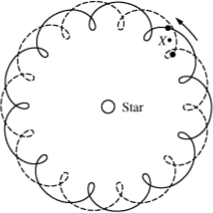
\includegraphics[height=.75in]{doubleplanet.png}
	\end{center}
The figure above represents the orbits of two planets of equal mass that orbit their star in the counterclockwise direction as a double-planet system. From the point of view of an observer on either planet, the planets appear to orbit each other while also orbiting the star. The dots on the orbits represent the position of the planets at time t\textsubscript{0}, and X is the position of their center of mass at that time. Which of the following arrows best represents the acceleration of the center of mass of the double-planet system when it is at point X?
 \choice{$\nwarrow$}
 \choice{$\swarrow$}
 \choice{$\nearrow$}
 \choice{$\searrow$}
\end{question}




%\begin{question}
%Two satellites are in circular orbits around Earth. Satellite A has speed $v_A$. Satellite B has an orbital radius nine times that of satellite A. What is the speed of satellite B?
%
%	\choice{$\frac{v_A}{9}$}
%	\choice{$\frac{v_A}{3}$}
%	\choice{$3v_A$}
%	\choice{$9v_A$}		
%	\end{question}
\end{multiplechoice} 


%\begin{shortanswer} [title={Free Response},	rearrange=no]
%	\begin{question}
%		Jupiter has a mass of 1.898 x 10\textsuperscript{27} kg.  It's moon Io is 4.217 x 10\textsuperscript{8} m.  How long does it take Io to orbit Jupiter, in hours?  \vspace{1in} 
%	\end{question}
%	
%\end{shortanswer}




\begin{truefalse} [title={True or False},
	rearrange=no]
	\begin{question}
		\answer{false} 9. The Sun's gravity pulls on the Earth more than the Earth's gravity pulls on the Sun.  
	\end{question}
	\begin{question}
		\answer{false} 10. The Moon has no gravity.
	\end{question}

	\begin{question}
	\answer{false} 11. A planet's gravity is caused by its atmosphere alone.
\end{question}

	\begin{question}
	\answer{false} 12. Planets distant from the Sun have less gravity.
\end{question}

	\begin{question}
	\answer{false} 13. Gravity is stronger between the most distant objects.
\end{question}

	\begin{question}
	\answer{false} 14. Space shuttle astronauts are weightless because there is no gravity above earth.
\end{question}


\begin{question}
	\answer{false} 15. Planets revolve around the sun because they are pushed by gravity.
\end{question}



\begin{question}
		\answer{false} 16. The gravitational field of the Earth is infinite in size. 
	\end{question}
		


\end{truefalse}







\end{document}


